
基于事件的系统,是那些架构围绕着事件处理的系统。有生成事件的组件、传播事件的通道和响应事件的侦听器,也可能触发新的事件。这种风格更加异步和低耦合,使得其成为提高性能和可扩展性的好方法,同时也是一种易部署的解决方案。

除了这些优势,还有一些挑战。其中之一是创建这类系统的复杂性。所有队列必须具有容错功能,以便事件在处理过程中不会丢失。以分布式方式处理事务也是一个挑战。使用关联ID模式跟踪进程之间的事件,以及监视技术,可以节省调试时间和思考的时间。

基于事件的系统包括流处理器和数据集成,以及以低延迟或高可扩展性为目标的系统。

现在让我们讨论一下此类系统中常见的拓扑结构。

\subsubsubsection{2.5.1\hspace{0.2cm}基于事件的拓扑}

事件驱动体系结构有两种主要拓扑:基于代理和基于中介。这些拓扑的不同之处在于事件在系统中的走向。

中介拓扑,适合用于处理需要多个可独立执行的任务或步骤的事件。最初,产生的所有事件都需要放在中介的事件队列中。中介器知道为了处理事件需要做什么,会通过每个处理器的事件通道将事件分派给相应的事件处理器。 

敏感的读者可能会突然想到,这是关于“业务流程是如何流动的”话题。当然,可以在业务流程管理(BPM)或业务流程执行语言(BPEL)中实现此拓扑。并且,也可以使用Apache Camel、Mule ESB等方式进行实现:

\begin{center}
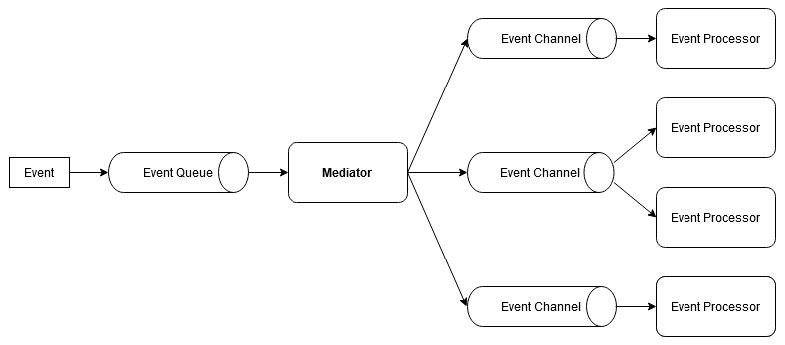
\includegraphics[width=0.8\textwidth]{content/1/chapter2/images/1.jpg}\\
图2.1 - 中介拓扑
\end{center}

另一方面,代理是轻量级组件,包含所有队列,不协调事件的处理。可以要求收件人订阅特定类型的事件,然后简单地转发他们感兴趣的事件。许多消息队列依赖于代理,例如ZeroMQ,用C++编写,目标是零浪费和低延迟:

\begin{center}
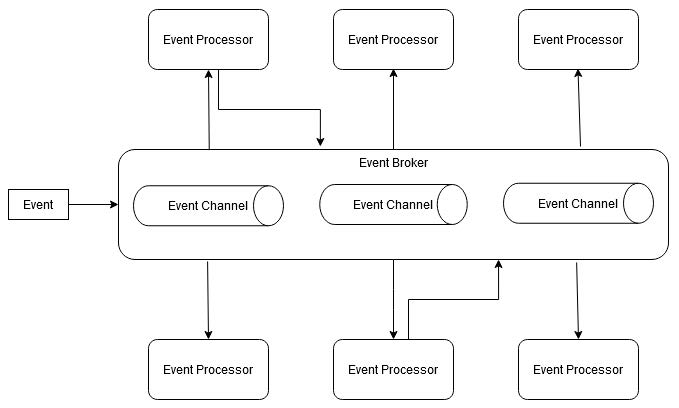
\includegraphics[width=0.8\textwidth]{content/1/chapter2/images/2.jpg}\\
图2.2 -代理拓扑
\end{center}

现在,已经了解了基于事件的系统中使用的两种常见拓扑,接下来让看下以事件为核心的架构模式。

\subsubsubsection{2.5.2\hspace{0.2cm}事件源}

可以将事件视为通知,其中包含要处理的通知服务所需的数据。还可以以另一种方式来看——状态的改变。若能够知道错误发生时的状态,以及需要进行的更改,那么用应用程序逻辑调试就会很容易。这是事件源的一个红利,它通过简单地按照事件发生的顺序记录所有事件,捕获发生在系统上的所有更改。

通常,会发现服务不再需要将其状态存到数据库中,因为将事件存储到系统的某个地方就足够了,也可以异步完成。从事件源中获得的另一个好处是免费的完整审计日志:

\begin{center}
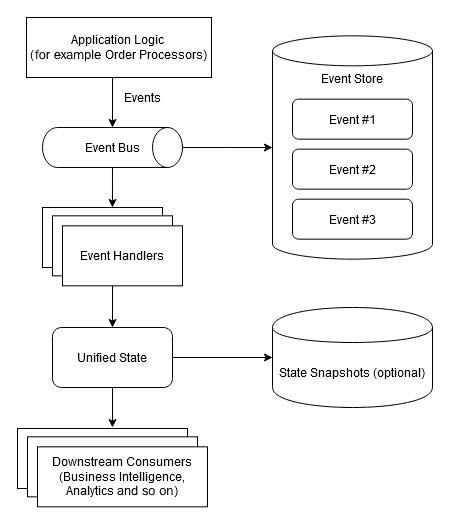
\includegraphics[width=0.8\textwidth]{content/1/chapter2/images/3.jpg}\\
图2.3 - 事件源架构提供应用程序状态的统一视图,可以使用该视图并创建定时快照以实现快速恢复
\end{center}

由于减少了对数据同步的需求,事件源系统通常提供较低的延迟,所以更适合交易系统和活动跟踪器。

接下来,了解一下另一种流行的架构风格。






















